This section shows the results of the lastest prototype developed in the TRITIUM experiment, TRITIUM-IFIC 2, during its installation in the Nuclear Radiation Laboratory at IFIC. The design of this prototype is shown in section \ref{subsec:TritiumIFIC2}.

The energy spectra of the signal and background prototypes were measured, which are shown in Figure \ref{subfig:SignalBackgroundEnergySpectraTritiumIFIC2}. As it was mentioned in section \ref{subsection:TritiumIFIC2}, the signal prototype was filled with a tritiated water solution with an activity of $10~\kilo\becquerel/\liter$ and the background prototype was filled with ultrapure water.

\begin{figure}[h]
 \centering
  \subfloat[Signal and background energy spectra.]{
   \label{subfig:SignalBackgroundEnergySpectraTritiumIFIC2}
    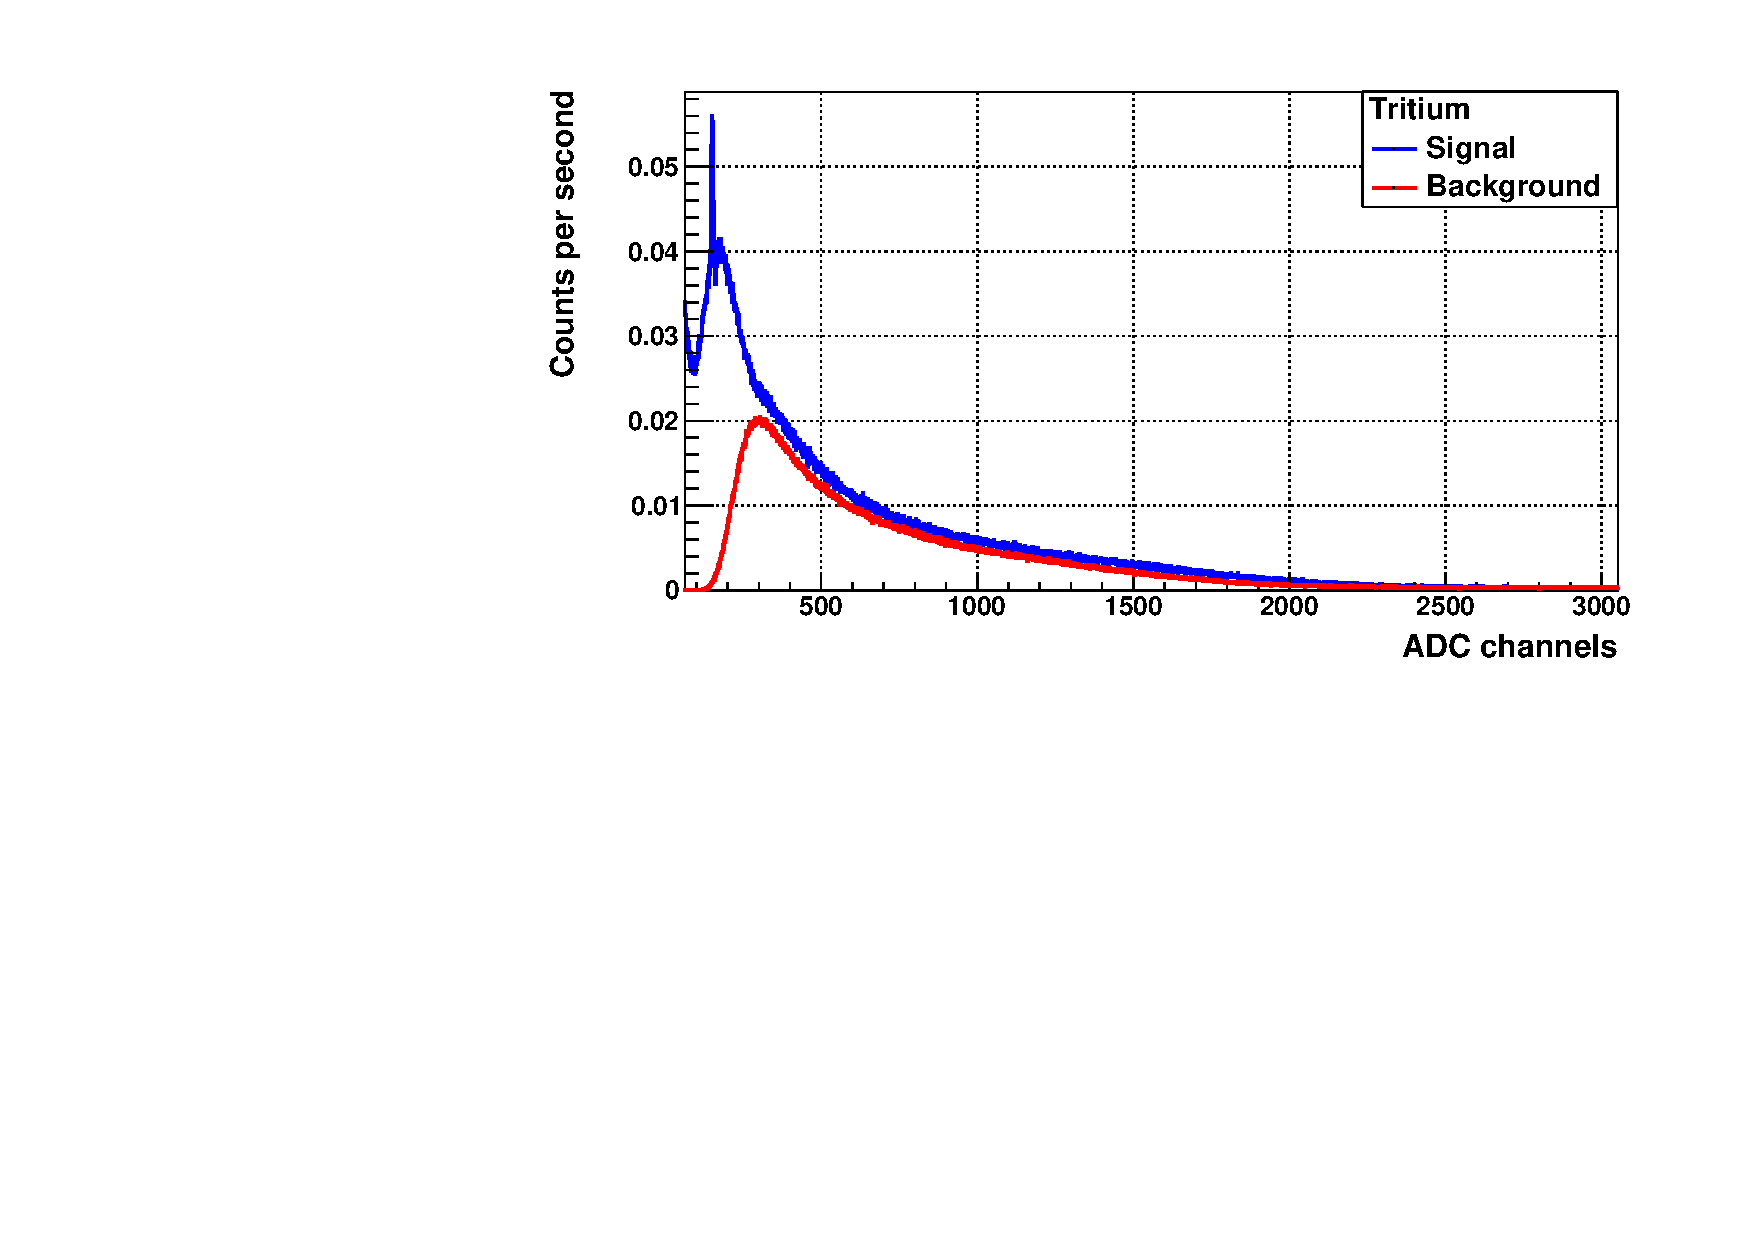
\includegraphics[width=0.73\textwidth]{7ExperimentalResultsDetectors/71ExperimentalResultsLaboratory/714TRITIUMIFIC2/TritiumIFIC2SignalsHigherZOOM.pdf}}
   \newline
  \subfloat[Tritium energy spectrum.]{
   \label{subfig:TritiumEnergySpectraTritiumIFIC2}
    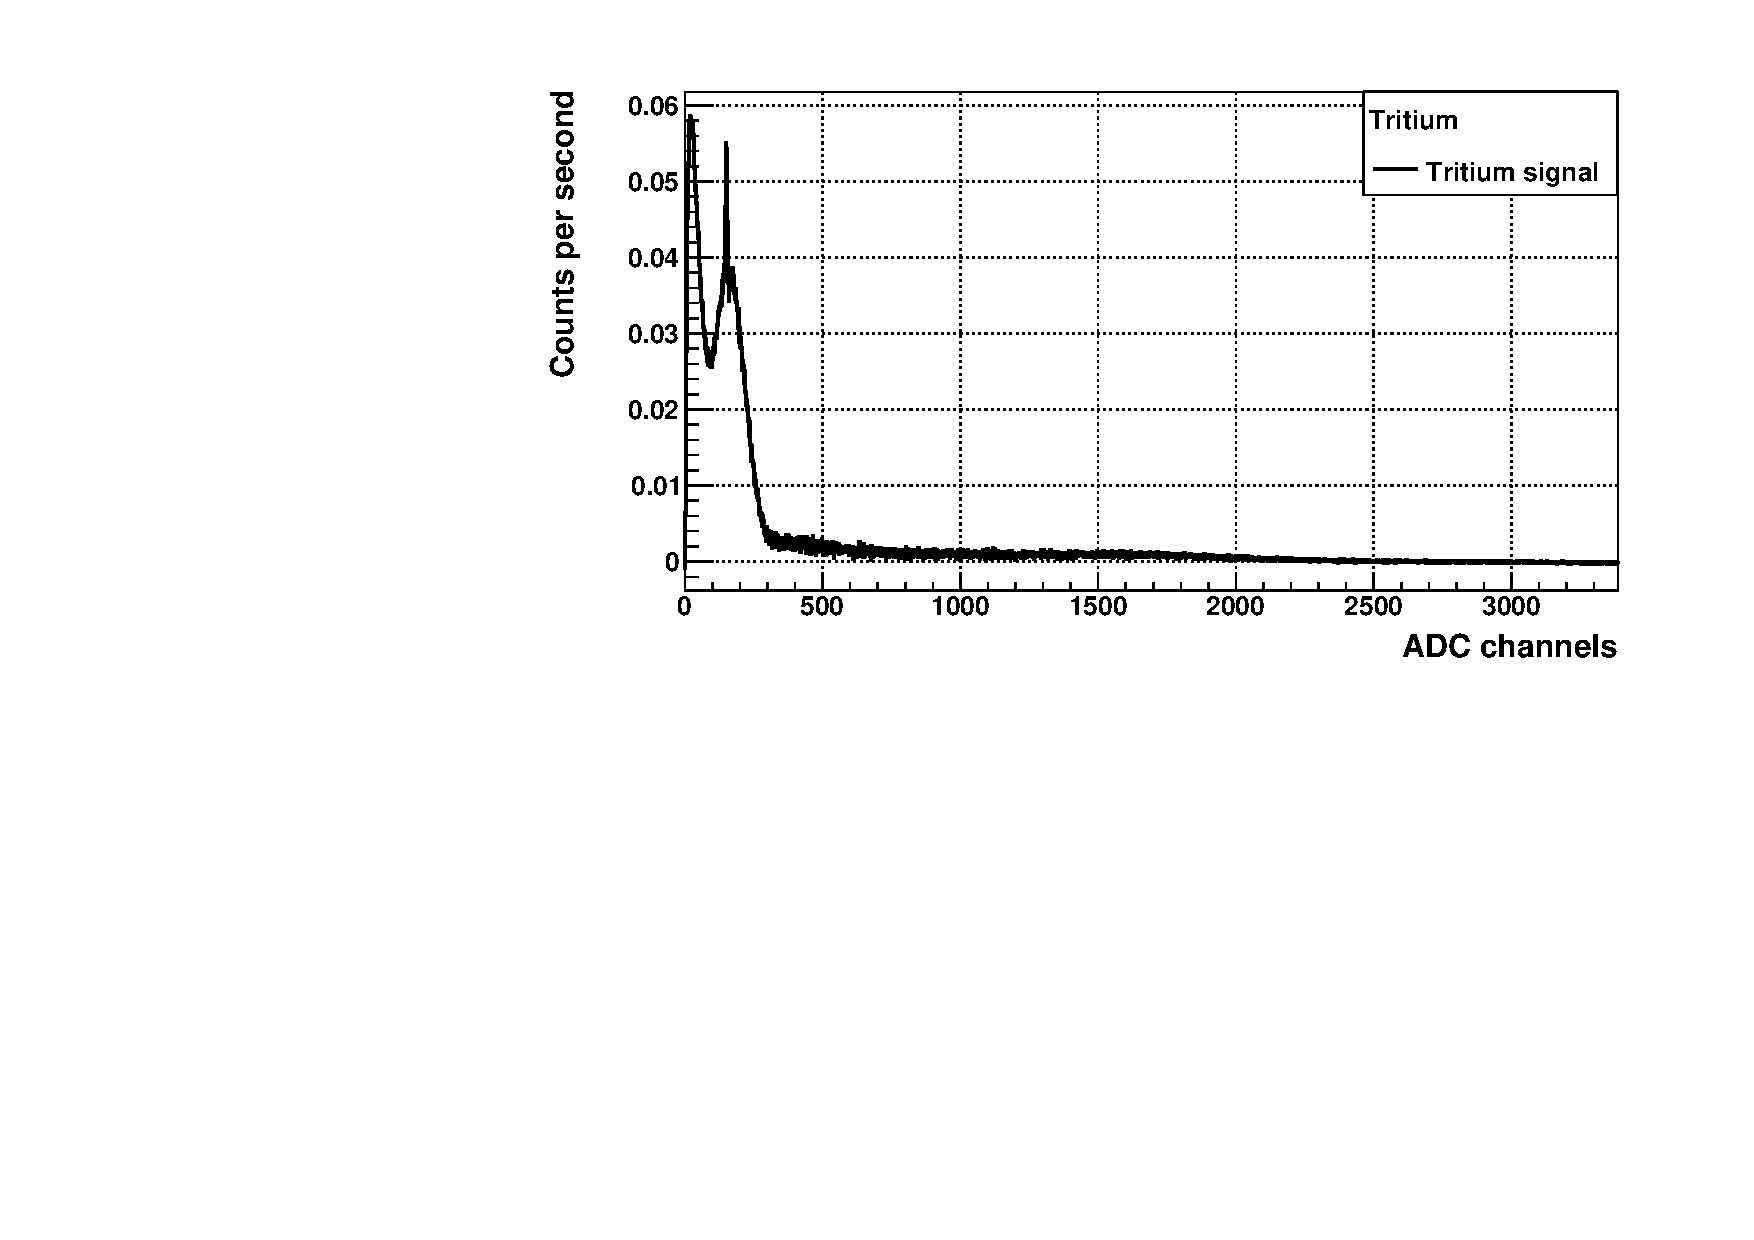
\includegraphics[width=0.73\textwidth]{7ExperimentalResultsDetectors/71ExperimentalResultsLaboratory/714TRITIUMIFIC2/TritiumIFIC2ClearHigherZOOM.pdf}}
 \caption{Energy spectra experimentally measured with TRITIUM-IFIC 2 prototype.}
 \label{fig:EnergySpectraTRITIUMIFIC2}
\end{figure}

A difference between both signals is clearly visible, which corresponds to the energy spectrum of tritium, Figure \ref{subfig:TritiumEnergySpectraTritiumIFIC2}. The number of counts per second obtained for both, the signal and background, are $19.05 \pm 0.18$ and $11.54 \pm 0.14$ respectively. Therefore, $7.11 \pm 0.23$ counts per second was obtained for the tritiated water source used.

The tritium detection efficiency obtained for this prototype is $(7.11 \pm 0.28)\cdot{} 10^{-1}~ \frac{\text{c}/\second}{\kilo\becquerel/\liter}$, calculated from the quotient of both, the counts per second measured and the specific activity o the tritium liquid source used. This efficiency is larger than all scintillating detectors developed so far, including the prototypes developed in TRITIUM experiment, Table \ref{tab:PlasticScinTritium} and sections \ref{subsec:ResultsTritiumIFIC0}, \ref{subsec:ResultsTritiumIFIC1} and \ref{subsec:ResultsTritiumAveiro}. It is an expected result since the active area used in this prototype is larger than those used in others.

To remove the effect of different active area, the specific efficiency is measured, obtaining a value of $(1.59 \pm 0.48)\cdot{} 10^{-5}~ \frac{\text{c}/\second}{\kilo\becquerel/\liter}\frac{1}{\cm^{2}}$ for this prototype. Again, it can be observed that this prototype has the largert specific efficiency obtained so far with a scintillating detector used for tritium detection.

Therefore, as it has demostrated, the intrinsec and specific efficiency obtained so far for scintillating detectors used for tritium detection has been exceeded with the last TRITIUM prototype, TRITIUM-IFIC 2.

As discussed in chapter \ref{chapter:Research and Development}, the energy spectrum is shown in ADC units, proportional to energy, since it is difficult, even impossible, to calibrate a plastic scintillator due to its large relative uncertainty in the number of photons produced per event. Nevertheless, a detector calibration can be performed to express the results in units of photons detected per event. It was carried out using the single-photon distribution of the used PMTs, which was obtained from their self-emissions. Similar to the TRITIUM-Aveiro 0 prototype, the PMT used to read this prototype was decoupled to the prototype and covered with a special black blanket to ensure that external photons did not reach the PMT. The output signal of the PMT was analized using the electronical chain, the design of which is shown in Figure \ref{subfig:ElectronicConfiguraiton1PMT}. The distribution measured is shown in Figure \ref{subfig:SinglePhotonDistributionIFIC2}, in which a gaussian function was fitted.

\begin{figure}[h]
 \centering
  \subfloat[Single photon distribution.]{
   \label{subfig:SinglePhotonDistributionIFIC2}
    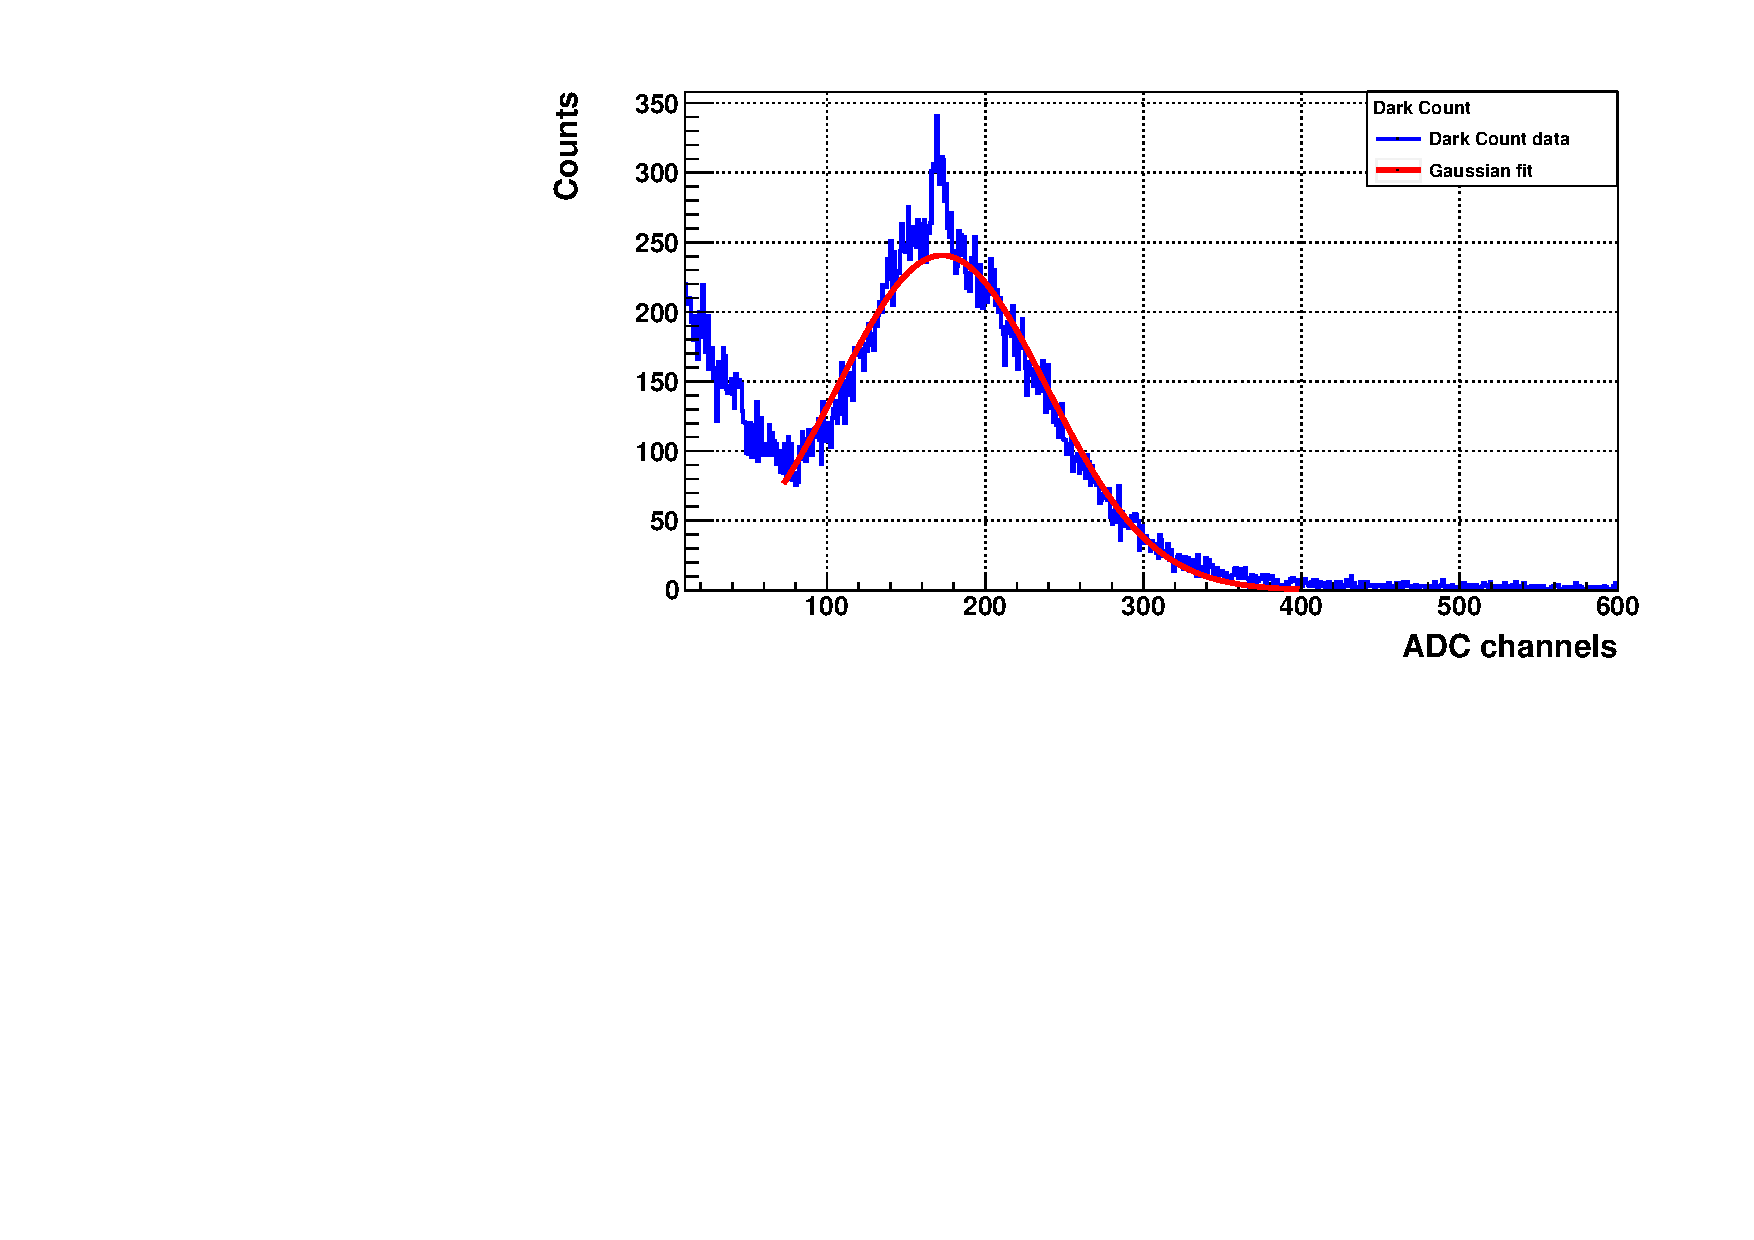
\includegraphics[width=0.73\textwidth]{7ExperimentalResultsDetectors/71ExperimentalResultsLaboratory/714TRITIUMIFIC2/SinglePhotonDistribution.pdf}}
   \newline
  \subfloat[Tritium energy spectrum.]{
   \label{subfig:TritiumSignalTRITIUMIFIC2}
    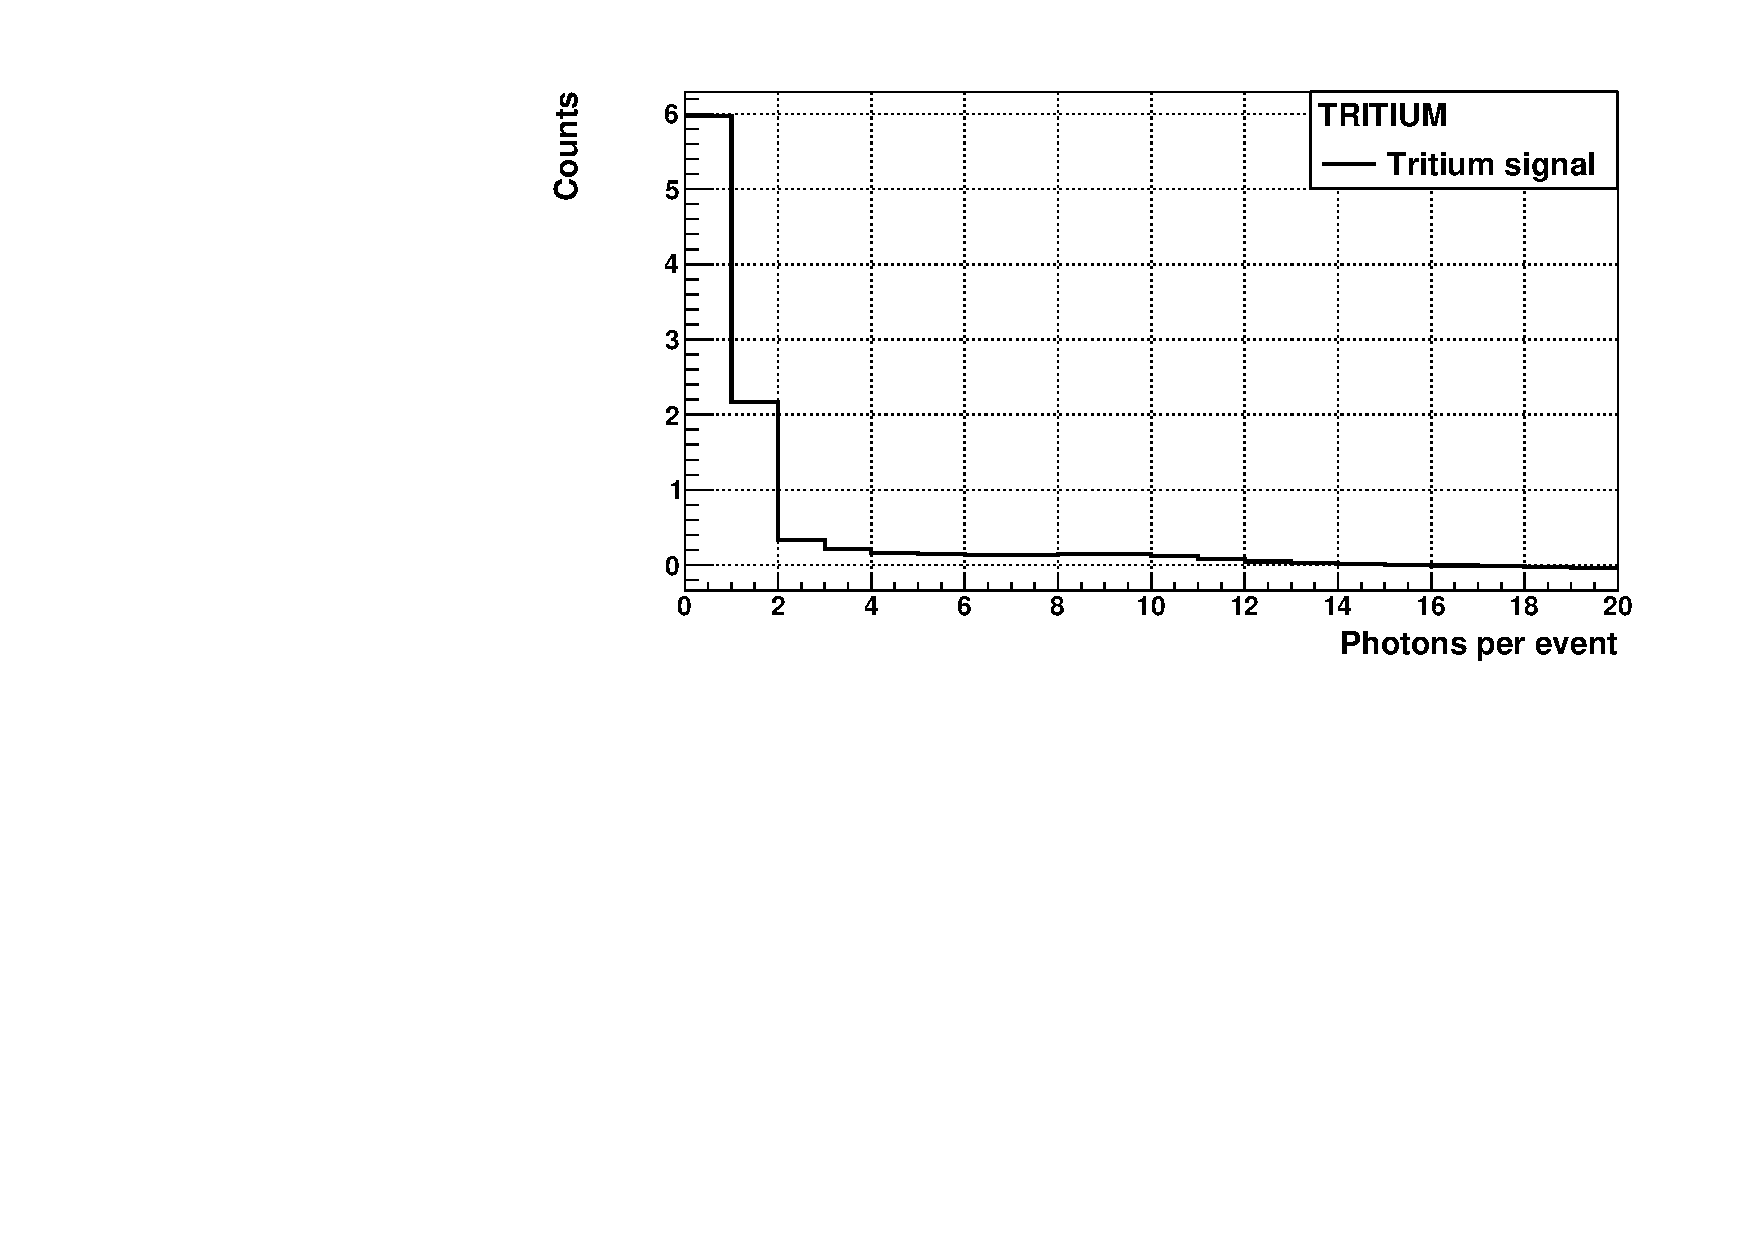
\includegraphics[width=0.73\textwidth]{7ExperimentalResultsDetectors/71ExperimentalResultsLaboratory/714TRITIUMIFIC2/PhotonsPerTritiumEvent.pdf}}
 \caption{Tritium measurement with TRITIUM-IFIC 2 prototype and expressed in photons detected per event.}
 \label{fig:PhotonsPerTritiumEventIFIC2}
\end{figure}

%\begin{figure}[h]
%\centering
%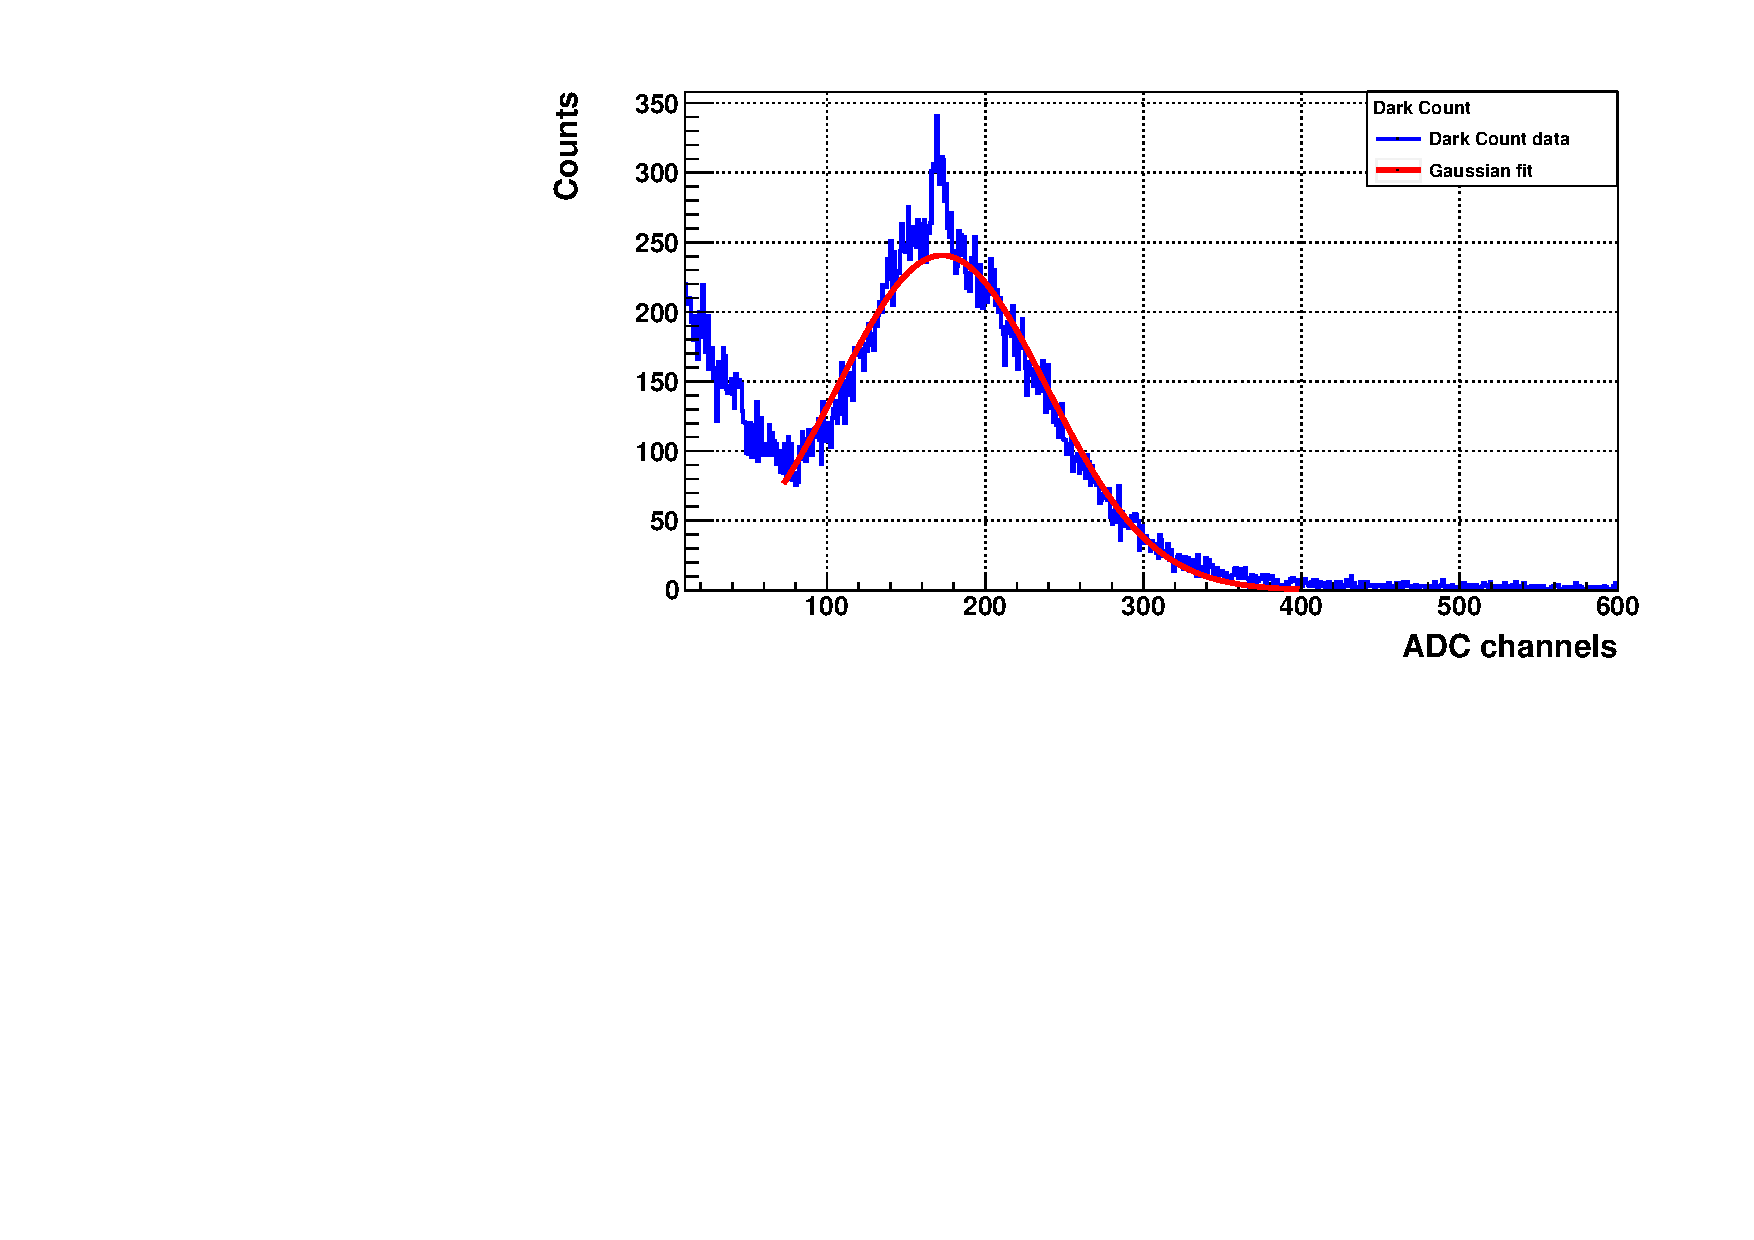
\includegraphics[scale=0.6]{7ExperimentalResultsDetectors/71ExperimentalResultsLaboratory/714TRITIUMIFIC2/SinglePhotonDistribution.pdf}
%\caption{Single photon energy distribution measured with the PMT used in TRITIUM-IFIC 2 prototype.\label{fig:SinglePhotonDistributionIFIC2}}
%\end{figure}

As can be seen, the mean and uncertainty of the signal produced for a single photon detected with the PMT used are $172.71$ and $66.19$ (in ADC units) respectively. Therefore, the tritium signal, Figure \ref{subfig:TritiumEnergySpectraTritiumIFIC2}, can be expressed in number of photons detected per event, Figure \ref{subfig:TritiumSignalTRITIUMIFIC2}, by simply dividing this spectrum by the mean measured for the single-photon distribution.

%\begin{figure}[h]
%\centering
%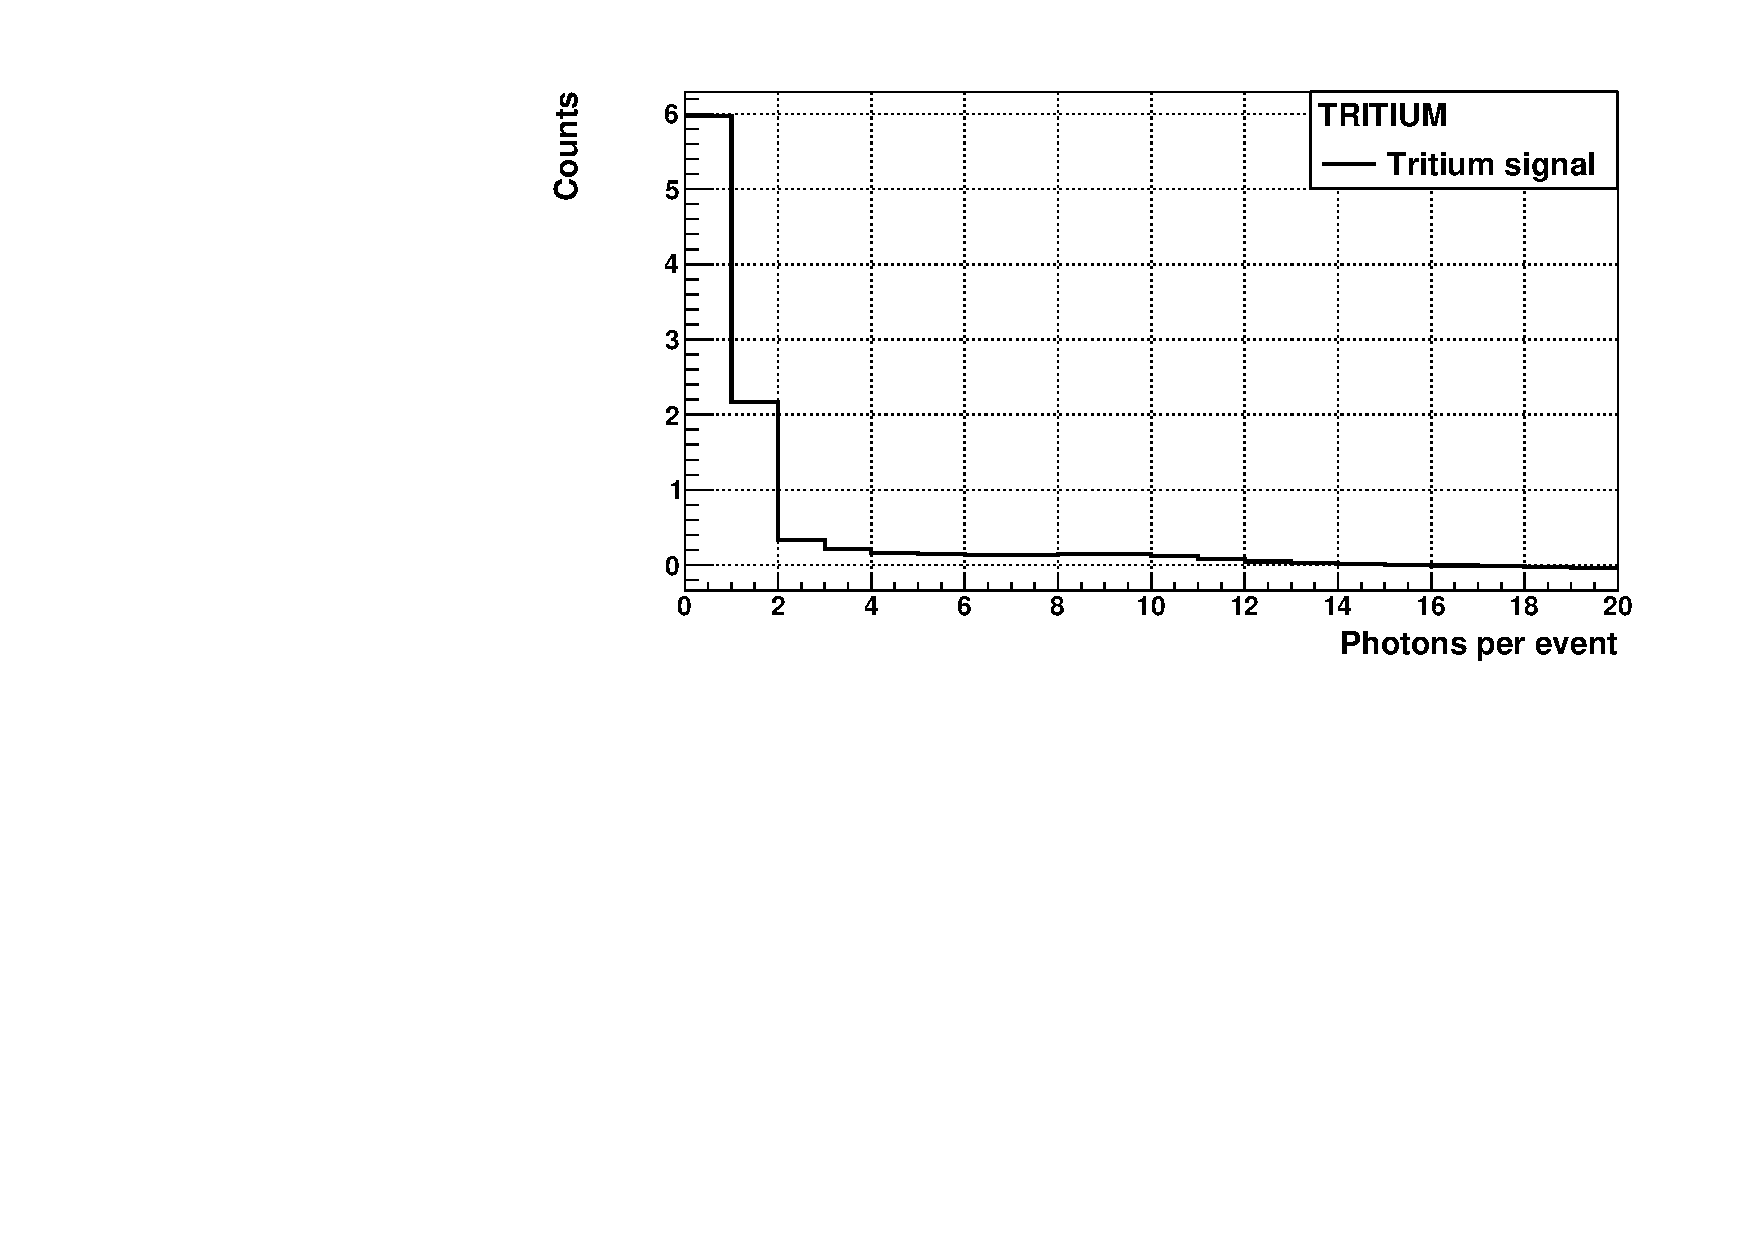
\includegraphics[scale=0.6]{7ExperimentalResultsDetectors/71ExperimentalResultsLaboratory/714TRITIUMIFIC2/PhotonsPerTritiumEvent.pdf}
%\caption{Tritium signal measured with the TRITIUM-IFIC 2 prototype and expressed in number of photones per tritium event detected.\label{fig:TritiumSignalTRITIUMIFIC2}}
%\end{figure}

As can be seen, a maximum of $15$ photons are generated per tritium event, which corresponds to the best situation. To compare the value obtained with the expected one, the different energies and efficiencies involved are taken into account. Considering a maximum energy for the tritium electron detected, $18.6~\keV$, a scintillation yield of $8000~\text{ph}/\MeV$ for the fibers, a maximum collection efficiency for the fibers, $7\%/\meter$, the fiber length, $20~\cm$ (which increases the collection efficiency by a factor of 5), and the PMT efficiency, $29\%$, the maximum number of photons produced for a tritium event detected with TRITIUM-IFIC 2 prototype is $15$. As can be seen, this is perfectly in accordance with the measurement.

Finally, a monitoring of both prototypes, signal and background, were carried out for several months, the measurements of which are shown in Figure \ref{fig:MonitorizationTRITIUMIFIC2}.

\begin{figure}[h]
\centering
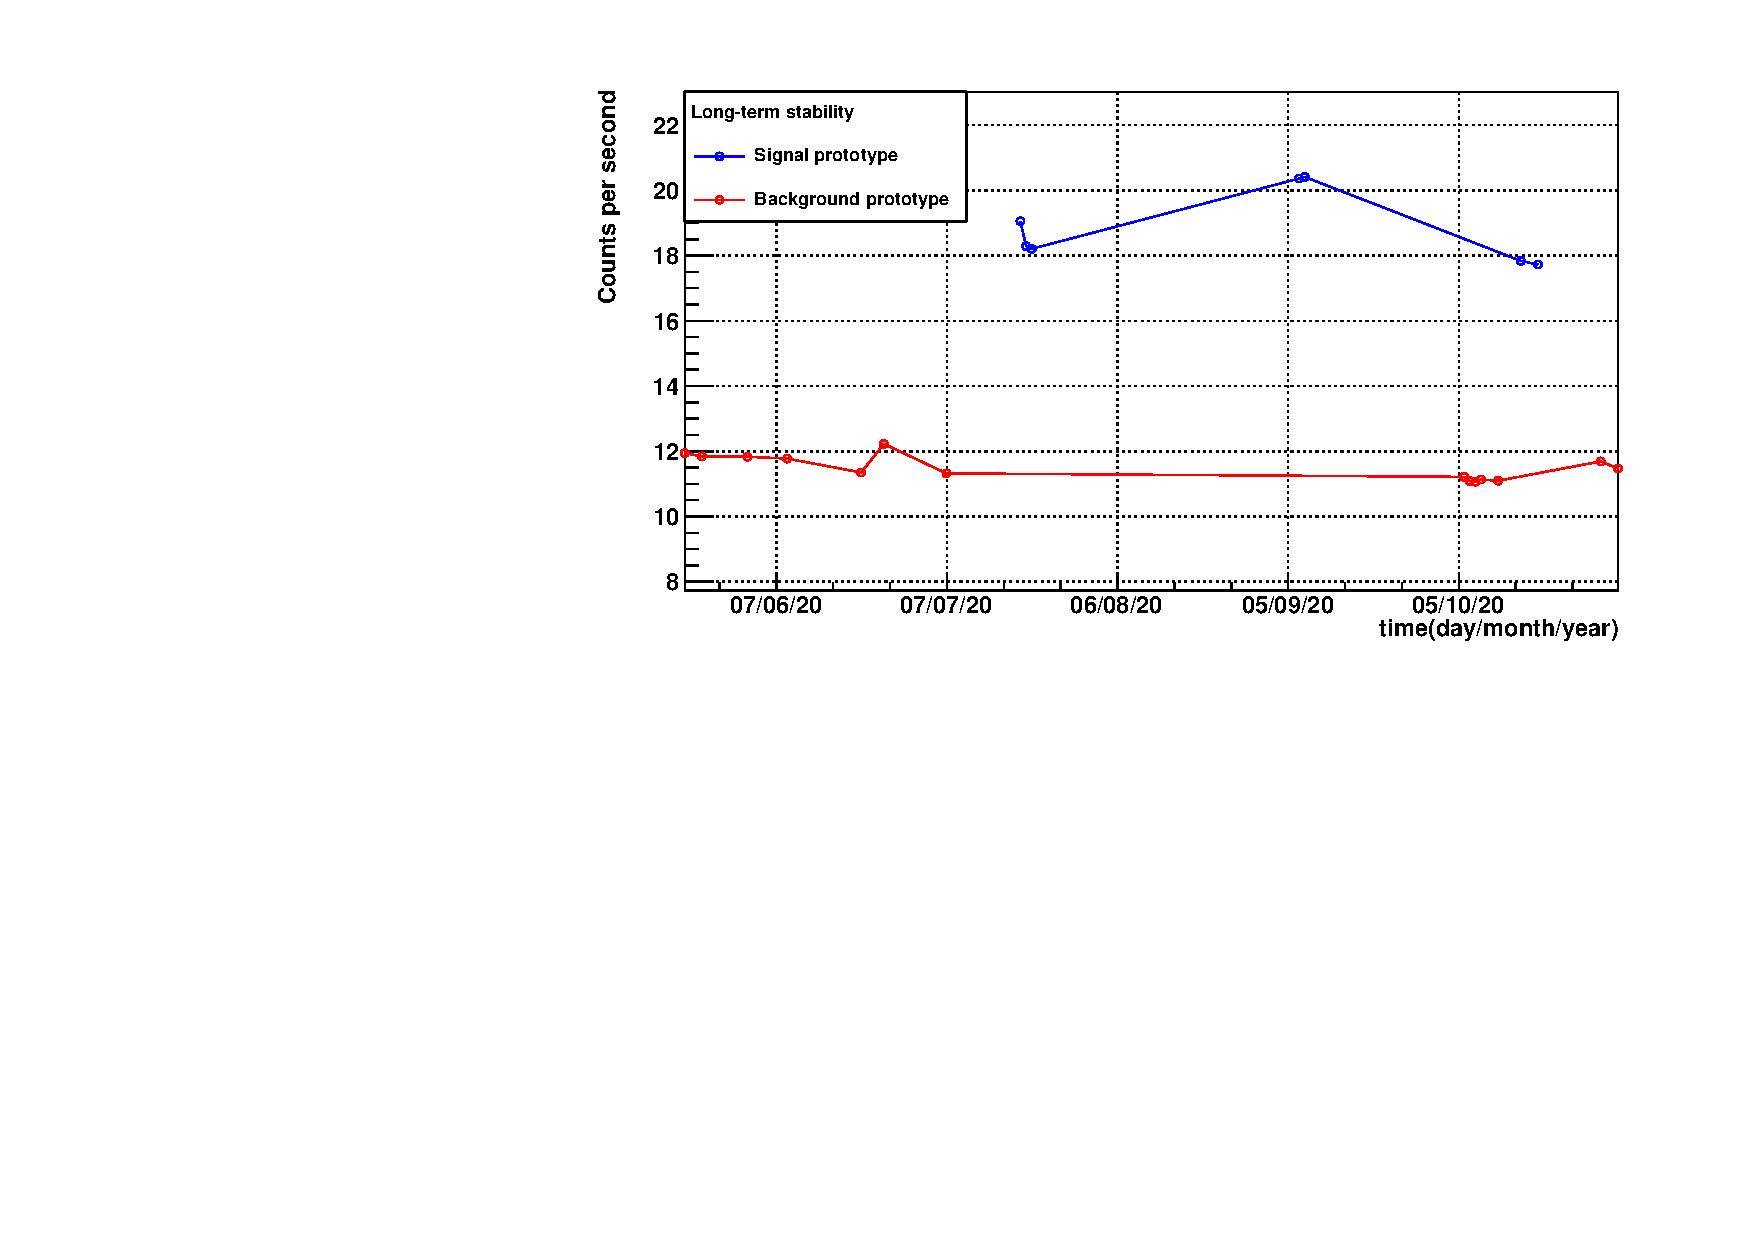
\includegraphics[scale=0.6]{7ExperimentalResultsDetectors/71ExperimentalResultsLaboratory/714TRITIUMIFIC2/Signal_Background_stability_ZOOM.pdf}
\caption{Monitoring of the signal and background prototypes for several months.\label{fig:MonitorizationTRITIUMIFIC2}}
\end{figure}

As can be seen, the signal of both was not reduced, ensuring the maintainance of the detector efficiency during 3 months for the signal and 6 months for the background.



%Rellenar con uan actividad grande y volver a medir. 

%Vaciar el prototipo y rellenar con actividades más pequeñas. 1000 y 100 Bq/L.

%Comparar fondos en el laboratorio, caceres, almaraz, etc.

%Medir en el prototipo con SIPM.

%Menos fondo que con el prototipo de AVEIRO en laboratorio Aveiro pero más que en laboratorio extremadura!!!!!!!!!!!!!!!!!!!!